%!TEX root = ../../thesis.tex

\subsection{Companion injection-recovery}
\label{subsec:injection-recovery}
To determine the detection limits for this method a injection-recovery approach was used to simulate spectra with a range of companions.
This is done by using the observed spectra and injecting onto them a synthetic companion, at the absolute flux ratio to which it would have been added to a synthetic host with the same parameters.
The {RV} of injected companion is set to 100\kmps{} so that the companion lines are well separated from the lines of the host.
This separation chosen is slightly larger than the largest host-companion separation ({HD~162020}) in the observed targets, given in \cref{tab:observations} \Rvtwo{}.

The search space for the injection-recovery is restricted by fixing the host parameters \(\teffsub{1}\) and \(\logg{}_{1}\) to those recovered fitting the non-injected spectra by a single component model.
This leaves only the companion \(\teffsub{2}\) and \Rvtwo{} parameters free, to recover the injected companion.
The wavelength masking is used to reduce the level of mismatch between synthetic and the observed spectra.
The spectra were injected with companions between 2500--5000\K{} and the companion recovery attempted on each.

The injection recovery also performed on a synthetic host spectra representing each target as a comparison.
For the synthetic host injection-recovery the wavelength range of the synthetic spectra used is three sections interpolated to 1024 values in the wavelength span of detectors \#1, \#2, and \#3.
For each section, Gaussian noise is added at the level measured in the corresponding detector in the observation of the target being represented.

In \cref{fig:injectrecoveryhd30501} the results of the injection-recovery on {HD 30501} are show the injected companion temperature verses the companion temperature recovered.
The blue dots represent the injection into the real observations, while the orange triangles represent injection into the synthetic host.
Error bars of \(\pm100\)\K{} are included to indicate the temperature grid size only, and do not come from the recovery itself.
The black dashed diagonal is the temperature 1:1 relation, where a correctly recovered companion should reside.

The grey shaded region indicates the \(\pm 1000\)\K{} temperature range explored for the injection-recovery of the companion.
This shows how the bounds of the grid can be recovered at low companion temperatures and that the recovered temperature deviates from the injected companion temperature around 3800\k{}.

For {HD 30501} the injection onto synthetic and observed spectra produce similar results.
At temperatures above 3800\K{}, in both the real and synthetic spectra, the injected companion is recovered within 100\K{}.
For injected companion temperatures below 3800\K{} the temperature recovered is systematically higher than the injected value.
This indicates that the companion is not correctly recovered and is affected by the added noise.
The temperature of deviation is deemed to be the upper temperature limit for the recovery by this method.
For the other stars upper limit from the injected observations could not be reliably determined, mainly due to spectral mismatch issues.
In these cases the results from the synthetic injection are used to derive a temperature recovery cut-off for each target, each simulated with the closest synthetic spectrum to the host star.

Using the temperature cut-off values, an upper mass limit is derived for the companions around our stars using the~\citet{baraffe_new_2015} evolutionary models, finding the closest point matching the spectral temperature cut-off and \(\logg{}=5.0\).
These values are given in \cref{tab:mass_limits} and are between 560--618~\Mjup{}.
The flux ratio between the cut-off companion spectra and the host star are also calculated, being between 5--15\% in this wavelength span.

%!TEX root = ../thesis.tex
\begin{table}
       \centering
  \begin{threeparttable}

       \caption{Upper mass limits of target companions assuming a companion \logg{}=5.0. Masses are derived from~\citet{baraffe_new_2015} evolutionary models using \(\teff{}\) and \logg{}. The flux ratio \(\rm F_2/F_1\) is  the absolute flux ratio between the cut-off temperature and the target host star.}

        \begin{tabular}{l c c c}
            \toprule
            Target & \txteff{} cut-off (K) & \(\rm F_2/F_1\) & Mass limit (\Mjup{})\\
            \midrule
            {HD 4747}     &  3\,900 & 0.084 & 598 \\
            {HD 162020} & 3\,900 & 0.147 & 598 \\
            {HD 167665} & 3\,800 & 0.054 & 560 \\
            {HD 168443} & 4\,000 & 0.094 & 618 \\
            {HD 202206} & 3\,900 & 0.075 & 598 \\
            {HD 211847} & 3\,900 & 0.079 & 598 \\
            {HD 30501}   & 3\,800\tnote{a} & 0.106 & 560 \\
            \bottomrule
        \end{tabular}
        \label{tab:mass_limits}
        \begin{tablenotes}[flushleft]
            \small
                \item [a] {From observed spectra }
        \end{tablenotes}
  \end{threeparttable}

\end{table}



\subsubsection{\texorpdfstring{\textchisquared}\ shapes}
\label{subsubsec:chi2_shapes}
To try and understand this recovered companions further investigation into the \textchisquared{} space was performed of the {HD30501} synthetic simulation.

In \cref{fig:injection_shape} the minimum \textchisquared{} contours achieved for each companion temperature in the grid, regardless of \Rvtwo{}.
This is done for seven different injected companion temperatures between 2500 and 4500\K{}.
For the higher temperature companions, the \textchisquared{} is parabolic in shape, recovering the correct temperature, as expected.
At lower temperatures there is a strong asymmetry in the \textchisquared{} with it flattening out on the lower temperature side.
The 1-, 2-, 3-\(\sigma\) values (with 2 degrees of freedom) of 2, 6 and 11 above the minimum \textchisquared{} are not shown in the bottom panel of \cref{fig:injection_shape} which is a close-up around the minimum \textchisquared{} as they are indistinguishable in the top panel due to the extreme \textchisquared{} y-scale.
The black vertical line indicates the 2300\K{} temperature limit of the {PHOENIX-ACES} models.

\begin{figure}
    \centering
    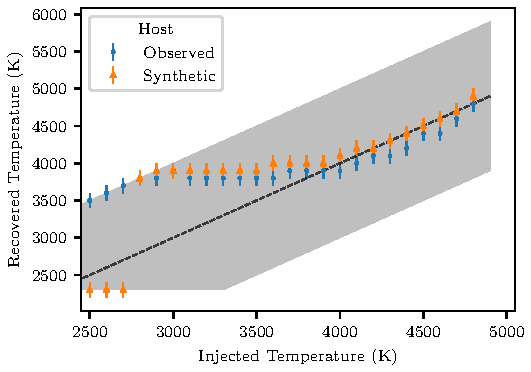
\includegraphics[width=0.6\linewidth]{figures/companion_recovery/inject_recovery_hd30501.pdf}
    \caption[Result of simulated injection-recovery of synthetic companions on {HD~30501}.]{Result of simulated injection-recovery of synthetic companions on {HD~30501}.
        The blue dots and orange triangles indicate the recovered companion temperature for the observed and synthetic spectra respectively.
        The \(\pm100\)\K{} error bars are the grid step of the synthetic models.
        The black dashed diagonal shows the 1:1 temperature relation.
        The grey shaded region indicates the \(\pm1000\)\K{} temperature range explored.
        Gaussian noise added to the synthetic spectra was derived from the observed spectra.}
    \label{fig:injectrecoveryhd30501}
\end{figure}


\begin{figure}
    \centering
    %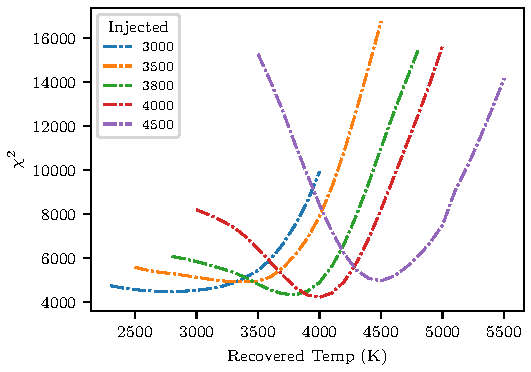
\includegraphics[width=0.7\linewidth]{figures/companion_recovery/chi2_shape_investigation}
    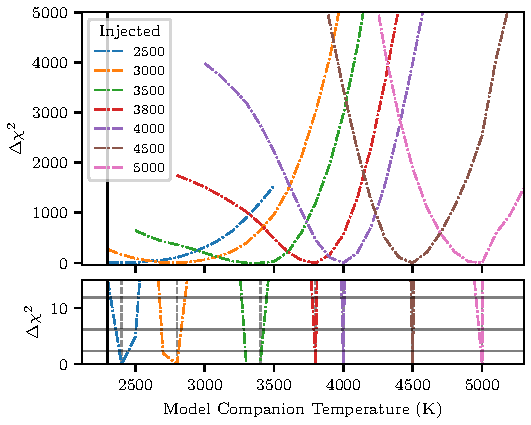
\includegraphics[width=0.7\linewidth]{figures/companion_recovery/chi2_shape_investigation_with_delta}
    \caption[Shape of simulated \textchisquared{} with different injected companion temperatures.]{Top: Companion temperature verses \textchisquared{} for simulations with different injected companion temperatures.
        The other fixed parameters for these fully synthetic simulations was \(\teffsub{1}=5200\)\K{}, \(\logg_{1}=4.5\), \(\logg{}_{2}=5.0\), and both \feh{}=0.0.
        A fixed Gaussian noise corresponding to a \snr{} of 300 was used.
        Bottom: A close up view of \textchisquared{} below 15.
        The three horizontal grey lines indicate the 1-, 2-, 3-$\sigma$ with 2 degrees of freedom.
        The vertical dotted lines indicate the location of the minimum \textchisquared{} recovered for each companion.
        The black solid vertical in both panels shows the 2300\K{} cut-off of the {PHOENIX-ACES} models}
    \label{fig:injection_shape}
    %\label{fig:chi2shapeinvestigation}
\end{figure}

